\section{Implementation, Integration and Test Plan}

\subsection{Overview}

The aim of this chapter is to show how to implement the system, then how to integrate the various components with each other and finally how to plan the test phases, in order to offer simplifications during the development of the whole system.
\\First, there is a description about how to implement, integrate and test single components. After that, the second step consists in defining the methods to follow to test the whole system and last there are some concerns about additional information regarding the testing process.

\subsection{Implementation, Component Integration and Testing Plan}

Here is a summary regarding the components that together constitute the CKB system:

\vspace{0.5cm}

\begin{itemize}
    \item \textbf{Web Server}
    \item \textbf{CKB Server}
    \begin{itemize}
        \item \textbf{CKB's Account Manager}
        \item \textbf{Search Helper}
        \item \textbf{Profile Viewer}
        \item \textbf{Tournament Viewer}
        \item \textbf{Tournament Manager}
        \item \textbf{Battle Manager}
        \item \textbf{Badge Helper}
        \item \textbf{CKB Notification Service}
    \end{itemize}
    \item External components
    \begin{itemize}
        \item \textbf{Github API}
        \item \textbf{Email Provider API}
    \end{itemize}
    \item \textbf{Query Manager}
\end{itemize}

\vspace{0.5cm}

To implement the system, we decided to opt for a bottom-up approach. By focusing on individual components and building gradually, it yields a more modular and scalable design. This facilitates specific modifications without impacting the entire system. 
\\Moreover, it promotes adaptability and flexibility, enabling optimization of distinct parts without compromising the overall technical project.
\\To follow the bottom-up approach, we highlighted the difficulty level to implement each component and we also provided a development order based on the dependencies between each component with the others, leading to a decision about the sequence of steps of implementation, component integration and testing. 
\\In the following steps we assume that DBMS component is already implemented and available (it is not represented for simplicity), to focus on the main components and sub-components of CKB system. 

\begin{table}[H]
    \centering
    \begin{tabular}{|c|c|}
        \hline
        Order & Stage\\
        \hline
        0 &
        $[F0]$ DB Interaction\\
        \hline
        1 & 
        $[F1]$ User Notifications\\
        \hline
        2 & 
        $[F2]$ Create Account and Log in\\
        \hline
        3 & 
        $[F3]$ View Profiles\\
        \hline
        4 &
        $[F4]$ Search Features\\
        \hline
        5 &
        $[F5]$ Managing Battles\\
        \hline
        6 & 
        $[F6]$ Managing Tournaments\\
        \hline
        7 &
        $[F7]$ Tournaments and Battles Features\\
        \hline
    \end{tabular}
    \caption*{Features Identification - Server Side}
\end{table}

\vspace{1cm}

\subsection{Development Stages Definition}

Here is a description about the steps to follow to implement, integrate and test the components of the system following the features enumeration described above.
\\Each component uses a driver to simulate other components not already implemented.

\begin{enumerate}
    \vspace{1cm}
    \item \textbf{DB Interaction}: the first component that must be implemented in the system is Query Manager, that offers to almost all other components in CKB server an interface to communicate indirectly with the DBMS.
    \vspace{0.5cm}
    \begin{figure}[H]
        \centering
        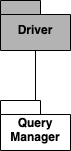
\includegraphics[scale=0.6]{src/phase0.drawio.png}
    \end{figure} 
    \vspace{0.5cm}
    \newpage
    \item \textbf{User Notifications}: this is the second step of the implementation and integration of components that satisfy the requirements for the CKB system. In this phase it's introduced and tested the Notification Manager to handle the notifications that the system sends to users. It offers interfaces to other components that will later be developed.
    \vspace{0.5cm}
    \begin{figure}[H]
        \centering
        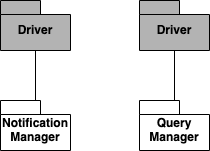
\includegraphics[scale=0.6]{src/phase1.drawio.png}
    \end{figure} 
    \vspace{2cm}
    \item \textbf{Create Account and Log in}: than component that have to be implemented is the one who manage the basic features to access the systems, that is creating a new account or logging in, with all the features that result from it, such as setting preferences or verifying an account whenever needed.
    The component that manages these features is CKB's Account Manager, the third one to be implemented and for which the unit tests have to be provided.
    Account Manager is integrated with Notification Manager as it leverages functionalities exposed by that component and with Query Manager to interact with DBMS.
    \vspace{0.5cm}
    \begin{figure}[H]
        \centering
        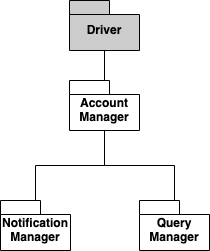
\includegraphics[scale=0.6]{src/phase2.drawio.png}
    \end{figure} 
    \vspace{0.5cm}
    \newpage
    \item \textbf{View Profiles}: the next phase consists in implementing and test Profile Viewer component, the one that manages user's profiles. It is integrated with Query Manager as it interacts with the DBMS to accomplish its operations.
    \vspace{0.5cm}
    \begin{figure}[H]
        \centering
        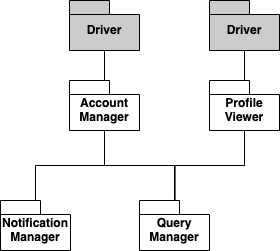
\includegraphics[scale=0.6]{src/phase3.drawio.png}
    \end{figure} 
    \vspace{2cm}
    \item \textbf{Search Features}: the next component that has to be implemented and tested is Search Helper. It offers the possibility to search for user profiles and to search for a tournament with filtering options.  It is integrated with Query Manager as it interacts with the DBMS to accomplish its operations.
    \vspace{0.5cm}
    \begin{figure}[H]
        \centering
        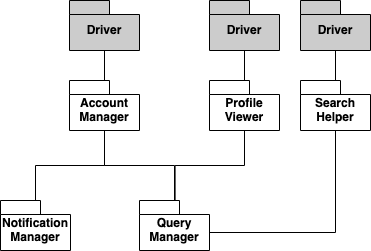
\includegraphics[scale=0.6]{src/phase4.drawio.png}
    \end{figure} 
    \vspace{0.5cm}
    \newpage
    \item \textbf{Managing Battles}: in this step must be implemented one of the core components for the system, Battle Manager. It offers an interface for the following component and it interacts with Account Manager so these two components have to be integrated.  It is integrated also with Query Manager as it interacts with the DBMS to accomplish its operations.
    \vspace{0.5cm}
    \begin{figure}[H]
        \centering
        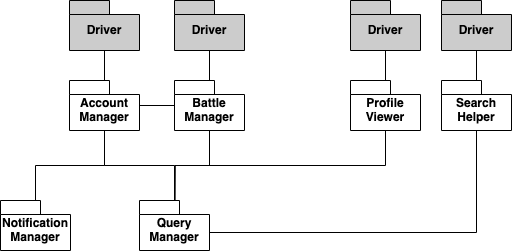
\includegraphics[scale=0.6]{src/phase5.drawio.png}
    \end{figure} 
    \vspace{0.5cm}
    \item \textbf{Managing Tournaments}: this is one of the most important feature of the system and the component that fulfill it is Tournament Manager, that offers all the features described previously in this document. Moreover, due to the possibility for educators to create badges before a tournament, in this phase is implemented also the Badge Helper component. Both components are integrated with Account Manager because many operations require the profile authentication to be executed. For both of these components must be provided the appropriate unit tests. The Tournament Manager component is also integrated with Battle Manager and Notification Manager to fulfill the main operations regarding the life cycle of a tournament. Finally, the component is integrated with Query Manager to interact with DBMS.
    \vspace{0.5cm}
    \begin{figure}[H]
        \centering
        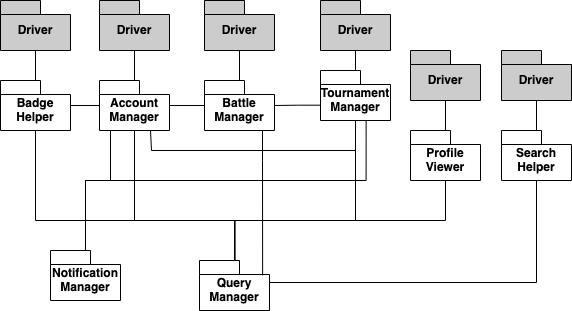
\includegraphics[scale=0.6]{src/phase6.drawio.png}
    \end{figure} 
    \vspace{0.5cm}
    \newpage
    \item \textbf{Tournaments and Battles Features}: this step implements and integrates in the system the Tournament Viewer component. It is integrated with Query Manager as it interacts with the DBMS to accomplish its operations.
    \vspace{0.5cm}
    \begin{figure}[H]
        \centering
        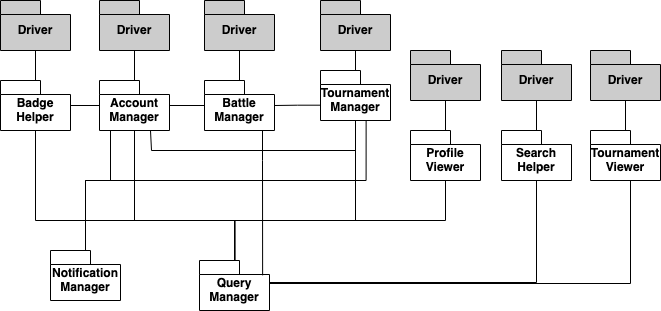
\includegraphics[scale=0.6]{src/phase7.drawio.png}
    \end{figure} 
    \vspace{0.5cm}
    \item \textbf{Dispatcher}: this component has to be implemented and tested to allow the correct interaction with different components.
    It's integrated with almost all the components previously described, so this phase is crucial to build and develop a working system. 
    \vspace{0.5cm}
    \begin{figure}[H]
        \centering
        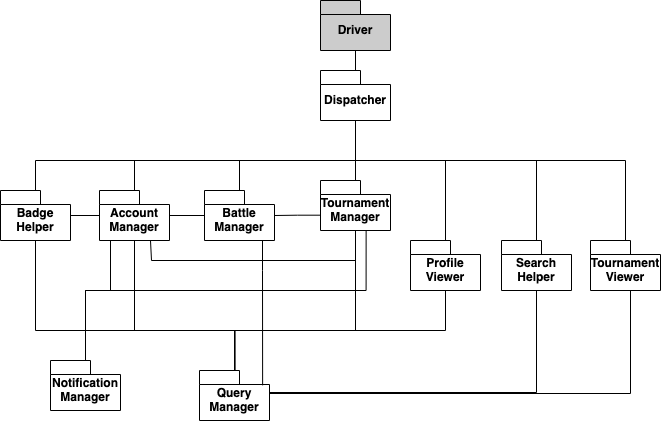
\includegraphics[scale=0.6]{src/phase8.drawio.png}
    \end{figure} 
    \vspace{0.5cm}
    \newpage
    From now on are implemented components to allow the communication between the client-side and the server-side.
    \vspace{2cm}
    \item \textbf{Web Server}: this component interacts from the server-side with the Dispatcher, so when the Web Server is implemented and tested, it has to be integrated with it.
    \vspace{0.5cm}
    \begin{figure}[H]
        \centering
        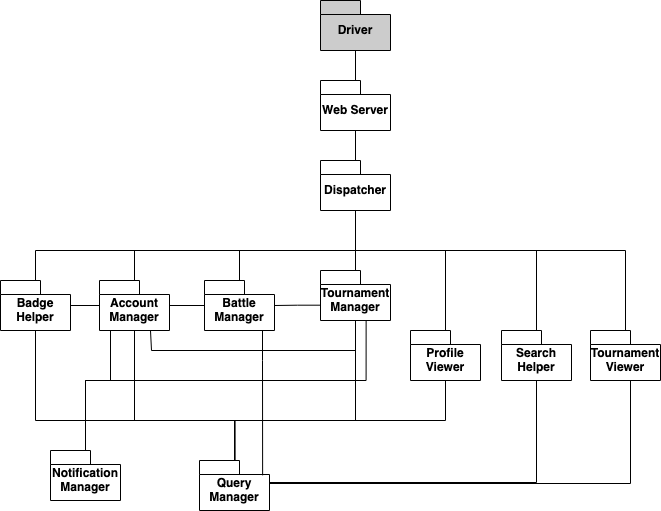
\includegraphics[scale=0.6]{src/phase9.drawio.png}
    \end{figure} 
    \vspace{0.5cm}
    \newpage
    \item \textbf{Web App}: this component represents the system on the client-side. It offers an interface to communicate with the server-side (it has to be integrated with Web Server). This interaction must be carefully curated down to the smallest details as it represents the main interaction between users and system.
    \vspace{0.5cm}
    \begin{figure}[H]
        \centering
        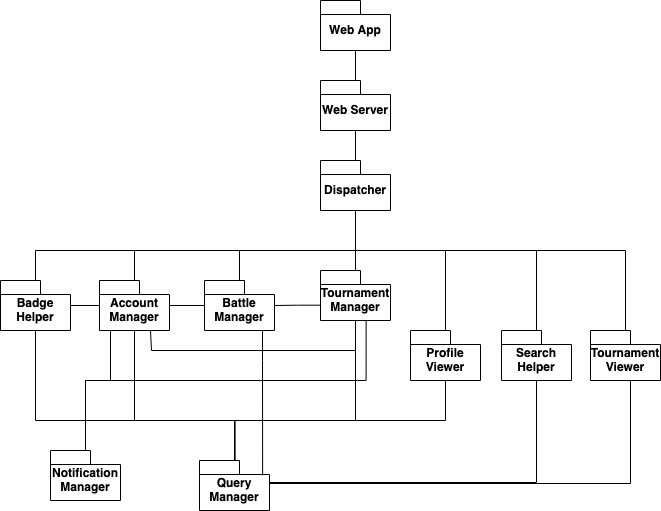
\includegraphics[scale=0.6]{src/phase10.drawio.png}
    \end{figure} 
    \vspace{0.5cm}
\end{enumerate}

\vspace{1cm}

\subsection{System testing}
\vspace{0.5cm}
This phase consider the system as a whole and concerns the testing of all the functionalities that the system has to fulfill, analyzing the requirements defined in the RASD. 
\\System testing is a more complicated step with respect to unit testing, and has to be performed by developers but with also an interaction with stakeholders, to make sure that the system is as close as possible to the desired final product.
\\
\\Different system testing techniques can be adopted and executed:
\begin{itemize}
    \item \textbf{Functional testing}: to check whether to software meets the requirements.
    \item \textbf{Performance Testing}: to highlight bottlenecks and measure response time and throughput and also hardware and network issues. To do so the testers have to load the system with expected workload and compare performances.
    \item \textbf{Load Testing}: to highlight bugs concerning the memory usage. To do so the testers have to load the system with increasing workload and for a long period.
    \item \textbf{Stress Testing}: to make sure that the system recovers gracefully after failure. The testers have to try to break the system under test by overwhelming its resources or by reducing resources.
\end{itemize}

\vspace{1cm}

\subsection{Additional specifications on testing}
A key point that must be underlined is that this is only a first version of the CKB system, so whenever new functionalities or changes in the requirements are made, the developers must check as first thing the functionalities added, and then also executing integration tests and system tests that can find new bugs before releasing a new version of the system. 
\\Once more, during the whole process, is important having an interactions with the stakeholders to take right decisions to create the right product.
